\documentclass[openany]{now} % creates the journal version
% \documentclass{now}  % creates the book pdf version

% a few definitions that are *not* needed in general:
\newcommand{\ie}{\emph{i.e.}}
\newcommand{\eg}{\emph{e.g.}}
\newcommand{\etc}{\emph{etc}}
\newcommand{\now}{\textsc{now}}
\newcommand{\newpar}{\bigskip\noindent}

\usepackage{color}
\newcommand{\authornote}[3]{\marginpar{\tiny\color{#1}#2: #3}{\color{#1}{$\star$}}}
\newcommand{\jin}[1]{\authornote{red}{Jin}{#1}}
\newcommand{\emine}[1]{\authornote{green}{Emine}{#1}}
\newcommand{\paul}[1]{\authornote{blue}{Paul}{#1}}
\newcommand{\note}[1]{\textit{(#1)}}

\title{Offline Evaluation for Information Retrieval}

% THe following author list is tentative
\author{
	Jin Young Kim \\
	Microsoft \\
	jink@microsoft.com
	\and
	Emine Yilmaz \\
	University College London \\
	emine.yilmaz@ucl.ac.uk
	\and
	Paul Thomas \\
	Microsoft \\
	pathom@microsoft.com
}

\begin{document}

% the following settings can be set or left blank at first
%\copyrightowner{N.~Parikh and S.~Boyd}
% \volume{1}
% \issue{3}
% \pubyear{2014}
% \isbn{978-0521833783}
% \doi{1234567890}
% \firstpage{23}
% \lastpage{94}

\frontmatter  % title page, contents, catalog information

\maketitle

\tableofcontents

\mainmatter

\begin{abstract}
Offline evaluation characterizes an information retrieval (IR) system
% based on human judgments
without relying on actual users in a real-world environment. \paul{This suggests that lab studies are in scope.} Offline evaluation, notably test collection based evaluation, has been the dominant approach in IR evaluation and it is no exaggeration to say that shared evaluation efforts such as the TREC conferences
\emine{cite and expand?} \paul{probably no cites in the abstract}
have defined IR research over the years. The reason for this success lies in the ability to compare retrieval systems in a reusable manner.

%Recently, there has been several trends which necessitates the change in the role and method of offline evaluation.
Several recent trends however necessitate a change in the role and methods of offline evaluation. First and foremost, online search engines with large-scale user base has become commonplace, enabling online evaluation based on user behavior \paul{Doesn't this suggest offline evaluation doesn't matter? Tone this down?}. There are new endpoints for search, such as mobile phones and conversational agents, and the types of search results has diversified beyond a list of web documents to include other result types. Finally, crowdsourcing has provided ways for human judgments of any kind to be collected at a large scale. The overall outcome of this trend is the advent of new IR evaluation paradigms which are more user-centric, diverse and agile.
\emine{This feels like part of a paper, as opposed to a book}

This survey aims to provide an overview of recent research in IR evaluation pertaining to the trends above. We first introduce offline evaluation for IR, focusing on how it relates to other evaluation paradigms such as online evaluation. We also overview traditional offline evaluation for IR, and how recent trends have shaped the research so far. We then review research in offline evaluation on three levels: human judgments, evaluation metrics and experiment design. This organization will allow readers to follow recent developments in research from micro-level (human judgment) to macro-level (experiment). Finally, we discuss evaluation practice in industry, which has been a major driving force in research and development in IR.
\emine{Maarten mentioned that since this will be like a book we should not have statements like recently (if I remember correctly)}
\paul{Hmm---tricky. Isn't this whole effort motivated by recent changes? How should we describe them?}
\emine{It may be better to have an organizaiton like:
	* Importance of offline evaluation
	* Difference from online evaluation and why it is important
	* Components of offline evaluation
	* Finally, organization of the paper}
\paul{We more or less have this in \S\ref{sec:evaluation-paradigms}, I think, although probably each of the sections in Ch1 could be expanded}
\end{abstract}

\chapter{Introduction}
\label{c-intro}

In this chapter, we survey the area and lay conceptual foundations for the rest of the paper. We first provide an overview of different approaches to IR evaluation. We then focus on offline evaluation, explaining traditional approaches and recent trends. Finally, we introduce a conceptual framework and the outline for the rest of this paper. \note{15-20 pages} \paul{We have 10pp, is ``15--20'' realistic?}

\section{Evaluation Paradigms in IR}
\label{sec:evaluation-paradigms}

Evaluating a search system, or any system that supports information access such as recommendation or filtering, is a complex problem.
% in general.
The performance of a search system is dependent on various contextual factors, such as the task at hand, the user's preference, abilities, location and other characteristics, and even the timing of the interaction. Also, the ultimate source of ground truth, the user's judgment, is subjective, volatile, and often hard to come by.

\subsection{Offline vs. Online Evaluation}

In order to meet these challenges, IR researchers have built a rich evaluation tradition. Most of this work has been based on a few simplifying assumptions. The document collection is static and the user's information need is represented as a description or a keyword query. The user's judgments in situ are replaced with judgments collected post-hoc and from third parties, often in the form of binary or numeric-scale labels.

We can define this evaluation paradigm as \textit{offline evaluation} \citep{INR-009} in that the evaluation of the system can happen without requiring an actual user. This makes offline evaluation particularly suitable for early-stage evaluation of an IR system, when users are hard to come by. Another typical characteristic of offline evaluation is that the test collection (a set of tasks, judgments and documents) is 'reusable', in that once built it can be used to evaluate new systems; because many factors are controlled, evaluations are also commensurable across time and between researchers.

An evaluation paradigm contrasting with offline evaluation is called \textit{online evaluation}. In a recent survey on this topic, online evaluation is defined as the evaluation of a fully functioning system based on implicit measurement of real users' experiences of the system in a natural usage environment \citep{INR-XYZ}. That is, online evaluation directly employs user behavior in natural environment for evaluation.

\note{more details of online evaluation / and its popularity}

\subsection{Hybrid Approaches}

So far we have introduced two evaluation paradigms -- offline and online evaluation -- with distinctive characteristics. Offline evaluation is based on human judges \paul{really? How about ``\dots is based on abstractions of real users''?}, and has strengths in experimental control and reusability. Online evaluation is based on user behavior, and has strengths in fidelity and cost.

While these two approaches comprise the majority of evaluation efforts, there have been several approaches trying to find a middle ground. Click modeling \citep{chuklin2015click} and counterfactual online evaluation \citep{Li:2015, li2010contextual}, for example, re-use online user data for future evaluation. These approaches, while enabling the re-use of online user data, are still limited in that they are based on implicit user behavior. \paul{how is that a limitation? need to be explicit}

Another related line of work is user study-based evaluation \citep{Bron:2013, Liu:2014, Shah:2011}, which is widely used in interactive IR studies \citep{kelly2009methods}. In such work, a group of participants are typically brought into a lab environment and asked to perform a set of (usually predetermined) search tasks. It is common for this type of study to collect both behavior and labels from the participants to get a more complete picture of search activity. 

User studies bear similarities with offline evaluation in that they typically involve some form of explicit judgments, but their emphasis is more on understanding some aspect of users' search behavior, as opposed to comparative evaluation among search systems. However, the distinctions are getting blurred as search engines increasingly serve more complex set of results, and SERP (search engine results page) or session-level evaluation is drawing more attention. In fact, some recent research has tried to use task completion settings for system-to-system comparison \citep{Xu:2009}. We will return to this point in Chapter~\ref{c-human-judgment}.

\subsection{When to Use Offline Evaluation}

At this point, a reader may ask: when should we use online vs. offline evaluation? While online metrics are certainly valuable,
% and must-have,
there are reasons we may need explicit input from human judges. First, in initial stages of system development we simply might not have real users to study. More importantly, traces of behavior are often insufficient to measure a user's true satisfaction. 

As an example, let's take clicks on results for evaluating a search engine. While click is certainly an indication that user is interested in the result, it is not clear whether the clicked result actually led to satisfaction. Also, click is often concentrated on the top of the page, making it difficult to interpret. That is, the ambiguity and bias inherent in user behavior often make it hard to infer true quality of our products.

Another consideration is the reusability of the data collected. In offline evaluation, typically the label is collected at the level of individual information item (i.e., document) and the system is evaluated by its ability to put more relevant items on top. This means the labels can be reused to evaluate new systems that produce different rankings. By contrast, the data collected from online system is valid for the evaluation of the system user interacted with, and the data should be collected for every new system to be developed.
\emine{Actually there are more reasons than that. I will send a table that contain advantages/disadvantages and we might want to include that.}

\section{Offline Evaluation for IR}

\subsection{Traditional Approaches in Offline Evaluation}

The field of IR has rich tradition in evaluation. %Starting with the work of Cleverdon \cite{cleverdon67} and his Cranfield collection, IR evaluation followed a few 

Conceptual Model

- Labels/Metrics based on Query-URLs

- Test collections 

- Concept of relevance 

\newpar
History

- TREC and related evaluation venues \cite{INR-009}

- Refer to \cite{borlund2003} \cite{cleverdon67} \cite{voor:trec05}

\subsection{Recent Trends in Offline Evaluation}

So far we have looked at traditional approaches in IR evaluation. While this tradition has served the community well for the past few decades, there has been several trends which necessitates the change in the role and method of IR evaluation. In this section, we outline recent trends and delve into their implications for offline evaluation.\emine{``recent''}

\subsubsection{User-Centric Evaluation}
First and foremost, online search engines with large-scale user base has become commonplace, enabling online evaluation based on user behavior. This availability of user data has opened up possibilities to validate assumptions of offline evaluation with actual user data. Also, recent work on evaluation metrics \cite{} \cite{} have embraced online user data to tune parameters of the metrics.

The overall outcome of this trend is the advent of new IR evaluation paradigms which are more user-centric, diverse and agile. Here, being user-centric means that the evaluation process is based on a model of user behavior, or/and aims to improve user satisfaction or other user-visible measure such as engagement or task completion (\cite{scholer13}). 

There has been already new methodologies proposed to better estimate user satisfaction and behavior in judgment collection \cite{VermaY16, VermaYC16} or metric design\cite{YilmazSCR10, CarteretteKY11, ChapelleMZG09}. Also, several recent work looked at cross-metric correlation \cite{Al-Maskari2007} \cite{radl:comp10} which aim to align IR evaluation with user satisfaction or some proxy of it.

As a side note, there has been an increasing\emine{} efforts to combine online and offline evaluation. These include ways to use online user data for offline evaluation \cite{Li:2015} \cite{li2010contextual} \cite{chuklin2015click}, or ways to collect feedback directly from user \cite{Kim2016}. 

\note{mentions of user study / iir papers}

\subsubsection{Diverse Endpoints and Search Scenarios}

There are also new endpoints for search beyond desktop web browser such as mobile phone and conversational agents. This opened up a whole venue of research which focuses on different interaction method and user experience in respective endpoints. For instance, mobile device has much smaller screen dimensions and the interaction is based on touch, and conversational agents use natural language, often in voice, to interact with the user.

Even for web search itself, the types of search results has diversified beyond the list of web documents to include other results types such as images, videos, news and even direct answers. This diverse set of results types and user interface design breaks many assumptions of traditional IR evaluation, providing rich opportunities for exploration. In particular, many of these 'answers' can directly satisfy users' information needs on SERP, making it hard to apply click-based evaluation techniques \cite{Li2009GA} \cite{diriye2012leaving}.

IR evaluation research has responded to this needs with various lines of work. There has been increased\emine{} interests on whole-page evlauation and optimization \cite{Zhou:2012}, which encompasses wide variety of page elements beyond web results. %Side-by-side evaluation 

Task and Session-level evaluation \cite{KanoulasCCS11, CarteretteKHC14} also drew interests, with TREC tracks of the same name \cite{}. Finally, there has been a new line of work focusing specifically on mobile interfaces \cite{VermaYC16}, or evaluation of search with spoken agents \cite{Kiseleva:2016}.

\subsubsection{Crowdsourcing / Agile Evaluation}

These diverse new endpoints and scenarios for search required ways to collect labels in a more agile manner, because many of these services are new and exploratory by nature, with less investments compared to well-established ones like web search.

Fortunately, crowdsourcing services such as Amazon Mechanical Turk has provided ways for human judgments of any kind to be collected at an large scale. Accompanying this new data collection method is the challenge in quality control, since the labeling work is completed by a remote worker on the internet.

\note{more on crowdsourcing for IR research}
\emine{Should we define that crowdsourcing is and how it may be useful for offline evaluation?}

\section{Scenarios for Offline Evaluation}

We have outlined basic concepts and recent trends for offline evaluation so far. The goal of this paper is to provide a practical guide in conducting offline evaluation for both academic and industry practitioners. Since there can be various scenarios in conducting offline evaluation, here we outline possible ones which we cover in this paper.

In classical IR research, a typical evaluation scenario is to improve the performance of a system given a test collection and a pre-determined set of evaluation metrics. For instance, in TREC Web Track, participants are given a collection representative of the Web, and then asked to submit the results for their systems in designated format and due date, which then will be evaluated on metrics like NDCG \cite{Jarvelin:2002} or ERR \cite{ChapelleMZG09}.

While academic IR research has developed well-accepted evaluation practice as above, the situation is a lot more ill-defined and varied from practitioners' standpoint. There are multiple components in a modern IR system such as web search engine, and each requires different emphases and considerations. For instance, one can think of component-level (i.e., query suggestions) evaluation as opposed to system-level evaluation. 

Also, building a working system serving real users takes several stages of development. The evaluation at early stages of development would be more exploratory in nature, whereas at later stage the focus would shift to making ship decisions and so on. We can call the former \textit{information-centric} evaluation in that the goal is to collect information helpful for system development and debugging, where the latter can be considered \textit{number-centric} in that the goal is to get reliable performance numbers for decision making.

Another characteristics of IR evaluation in industry setting is that the evaluation is an on-going process which takes multiple iterations over the lifetime of the service, as opposed to one-off research project. This necessitates the development of so called \textit{evaluation pipeline} where any new system can be evaluation on a ongoing basis.  

Since the goal of this paper is to meet the need of practitioners as well as academic researchers, we describe decisions one needs to face in conducting offline evaluation across various scenarios outlined above. We also focus on considerations in designing a evaluation pipeline in industry setting at Chapter \ref{c-experiment}.

\section{General Framework for Offline Evaluation}

In this section, we describe a general framework for offline evaluation in detail. The goal is to propose a general framework which can encompass diverse set of scenarios outlined above. 

\subsection{Definitions}

First, here are a few definitions that will be used throughout this paper. These comprise the components of offline evaluation.

\paragraph{Search Task} A search begins with user's information needs, which we call a search task. Search task can be represented as a description of information needs, or queries user would have used in actual information seeking.

\paragraph{Judging Target} Judging target denotes a result produced by an IR system to be evaluated. It can be of any granularity -- a snippet, a web document, or entire SERP. 

\paragraph{Human Judgment} Human judgment is an assessment of \textit{judging target} by a human judge in the context of \textit{search task} over some dimension of quality. 

\paragraph{Evaluation Metric} Evaluation metric (or metric in short) summarizes judgments into a single score. The design of evaluation metric depends on the type of judgments being collected, and the model of user behavior.

\paragraph{Experiment} An experiment is a collection of judgments with a specific purpose. An evaluation metric summarizes the outcome of an experiment, and an appropriate statistical test needs to be accompanied to make a claim about the validity and reliability of the findings.
\emine{I am not sure what an experiment refers to here}
\paul{Can we refer to this as an \emph{evaluation}? ``Experiment'' has a particular meaning; and in particular, (a) we need not be varying anything when doing offline evaluation (so it's not experimental) and (b) when we do, this measurement/evaluation can be a part of the larger experiment. Calling this an ``experiment'' is I think wrong, it's a measurement tool/technique}

%\paragraph{Evaluation Pipeline} 

\subsection{Evaluation Process}
Given the components above, here we discuss the general process for offline evaluation. At a high level, offline evaluation is composed of three steps 1) judgment design 2) metric design 3) experiment design. Alternatively, you can consider the whole process in terms of collecting data (judgments), combining them into meaningful numbers (metrics), drawing conclusions (experiment). Now we discuss major considerations in each step.

\begin{figure}
	\begin{center}
		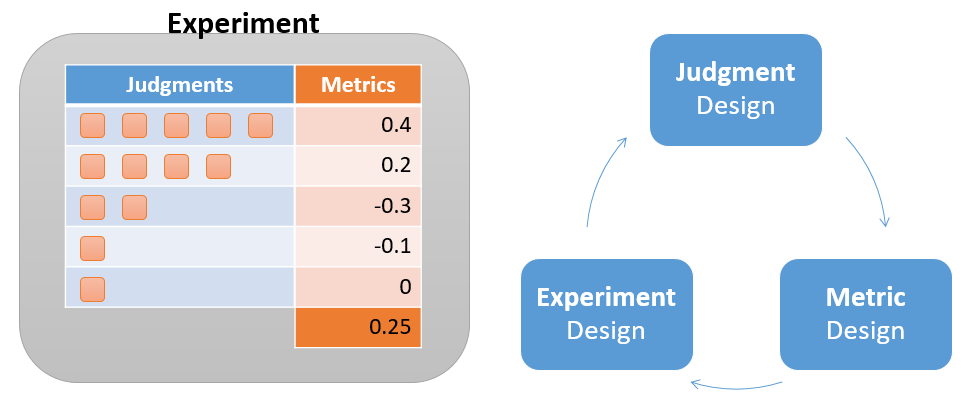
\includegraphics[scale=0.4]{images/offline_evaluation_overview}
		\caption{Overview of Offline Evaluation.} 
		\label{fig:offline_evaluation_overview}
	\end{center}
\end{figure}


%Offline evaluation for IR can be defined as the series of the following steps. We also list major decisions which need to be made for each step.


\subsubsection{Designing Human Judgments}

In the first step, the details of human judgment should be defined, which is the basic unit of offline evaluation. Here are major considerations in this step:\emine{Here we might want to summarize why we need human judgments, and what they simulate.}

\begin{enumerate}
	\item How do you define and collect search tasks?
	\item What should be your judging unit?
	\item How do you design judging interface?
	\item How do you hire and train judges?
\end{enumerate}

\subsubsection{Designing Evaluation Metrics}

The second step in offline evaluation is selecting or designing a meaningful evaluation metric. This is essentially the question of how to combine labels to meaningful numbers.

\begin{enumerate}
	\item How do you transform the labels from human judges?
	\item How do you define user models in combining labels into a metric?
	\item How do you estimate the parameters for the user model?
\end{enumerate}

\subsubsection{Designing and Running Experiments}

Lastly, judgments and metrics should be used to achieve the goal of evaluation. Since this is an iterative step which takes several stages of refinement, here we describe methods and criteria in doing so. 

\begin{enumerate}
	\item How do you size the experiment to fulfill your evaluation goal?
	\item How do you evaluate the outcome of the experiment?
\end{enumerate}


\section{The Organization of this Paper}

In the following chapters, we describe each process of offline evaluation in detail so that a reader can design his or her own evaluation pipeline following the flow of this paper. Chapter~\ref{c-human-judgment} deals with gathering judgments, which need to be created for the purpose. Chapter~\ref{c-metrics} considers steps in designing an effective metric. Chapter~\ref{c-experiment} covers the methods in designing and analyzing experiments. Finally, Chapter~\ref{c-practice} describes evaluation practices from major companies in search and recommendation area.
\emine{We already had a part describing the organization. In general, this section feels a bit repetitive given the text in first page}
\paul{I disagree, that was in the abstract; it makes sense here (as well) I think. Unless I missed something?}

\chapter{Human Judgments}
\label{c-human-judgment}

The goal of collecting a human judgment is to get an accurate measurement of  search engine results quality for given set of search tasks. A canonical example is collecting a binary relevance judgment for a document given a TREC-style search topic. The form of human judgment can be quite varied, however, depending on the type of search task and judging target.

We will start with an example to make the discussion more concrete. Figure~\ref{fig:human_judgment_overview} shows a list of possible search tasks about the topic of \textit{crowdsourcing} on the left side, and a few samples from existing web search results for query `crowdsourcing' on the right side.
\emine{Would it be better to show a more standard judging UI here? Like a query and a web page?}
\paul{Can we use another topic? We also discuss crowdsourcing below, which may be confusing. Let's use something which is clearly from a user not a researcher, e.g. ``rules of soccer''. I like the diagram otherwise I think}

\begin{figure}
	\begin{center}
		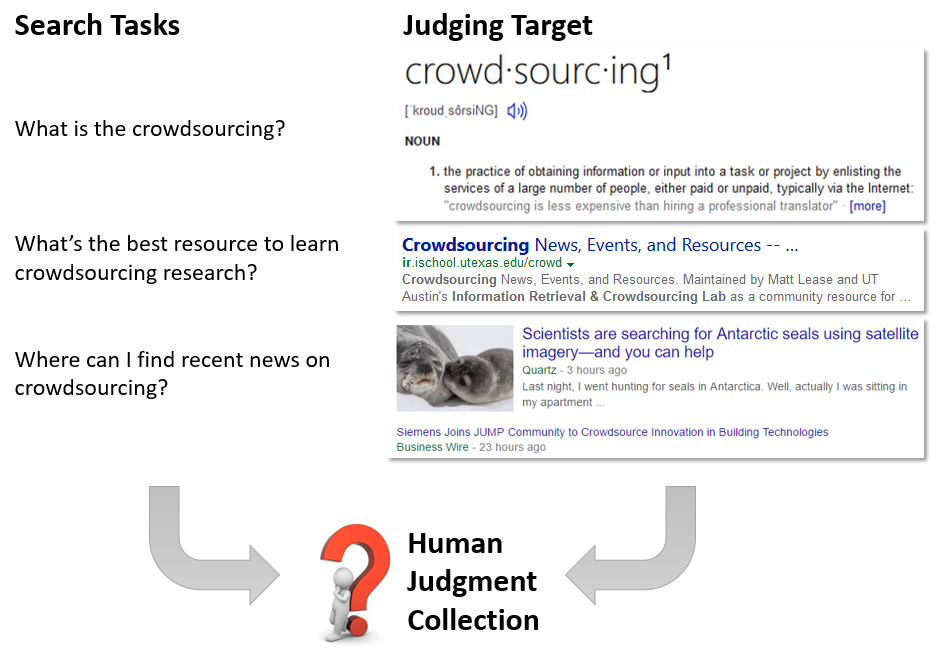
\includegraphics[scale=0.5]{images/human_judgment_overview}
		\caption{Overview of human judgment collection.} 
		\label{fig:human_judgment_overview}
	\end{center}
\end{figure}


This example presents basic ingredients in collecting human judgments -- search tasks and judging targets. From this example one can imagine a myriad of possibilities in designing a human judgment task. You can use either a (potentially ambiguous) keyword query or a well-defined topic description. You can collect judgment for a web document or any SERP element including instant answers or the list of news articles. 

The rest of this chapter is to give you guidance in designing a human judgment, in the light of recent literature on this topic. We will look over how to collect search tasks and how to determine a judging target. Various considerations in designing a judging interface will be examined. %, as well as the choice of judging resources.

%The first step in offline evaluation is collecting labels from human judges. In this chapter, we describe various considerations in collecting high-quality labels from human judges at scale. We first discuss the method for collecting search tasks, followed by the design of a judging method. We then discuss the collection of actual judgments, which is an non-trivial task to perform at scale. We also cover the trade-off and in using different types of judging resources -- in-house vs. crowd judges. (20-25 pages)


\section{Collecting Search Tasks}
Before considering judgment design, one needs to collect search tasks on which search results will be evaluated. Search tasks represents users' information needs that needs to be satisfied by the search results. In an industry setting where the search engine is used by actual users, the job of collecting search tasks can be as simple as sampling from queries users issued, whereas without access to such resources one needs to create tasks based on assumptions of target users and information needs. 

\subsection{Creating Search Tasks}
In many cases one needs to perform offline evaluation without a working system -- in building a new product, or in academic setting. It is essential to collect hypothetical search tasks in such cases, which is called simulated search or work (where work includes search and other things) tasks. \cite{Borlund:2003} summarizes the role of  simulated work task as follows:

% consider non-simulated search tasks?

\begin{quote}
A simulated work task situation, which is a short `cover story', serves two main functions: 1) it triggers and develops a simulated information need by allowing for user interpretations of the situation, leading to cognitively individual information need interpretations as in real life; and 2) it is the platform against which situational relevance is judged. Further, by being the same for all test persons experimental control is provided. Hence, the concept of a simulated work task situation ensures the experiment both realism and control.	
\end{quote}

`Task' can mean different things for different people, and IR literature has long debated over the definition of the search task, as summarized in \cite{kelly2009methods}. For our purpose, it is sufficient to understand it as the representation of information needs which a human judge can use to perform a search and\paul{and/or? Often no searching is done by a judge} judge the quality of results.
\emine{Is that the definition of task? May be we should use a more proper definition?}
\paul{task $\neq$ need, but I think this use is blessed by so much past use}

The design of search tasks needs many considerations which can critically affect evaluation results. First, there is the question of where the task is originated from and how much the judge is interested in the task. \cite{Edwards:2016} shows that judges' interests in the task has effects on how they perceive and perform the tasks. Judges in general had more knowledge on the tasks they were interested in, expected the tasks to be easier, and had higher engagement in terms of time spent.

Another dimension of task creation is the complexity, which again has many dimensions. \cite{Kelly:2015} looked at this problem using a cognitive complexity framework. They found that participants spent more efforts (queries, clicks and time to completion) in performing tasks with higher cognitive complexity (create, evaluate and analyze) than tasks with lower cognitive complexity (apply, understand, remember).

In sum, these results show that the characteristics of search task is an important dimension in designing an offline evaluation. It is recommended to collect information about task characteristics and design experiments accordingly so that one can control the effect of these factors in evaluation.

\emine{Should we talk about how to create the tasks?}
\paul{isn't that what we're doing?}

\subsection{Sampling Query Logs}
Assuming you have a working search engine with real users, it is natural to collect search tasks from query log data. While this is a seemingly straightforward task, there are a few considerations. We list these point below, along with recommendations based on recent studies.

\paragraph{Evaluation Goals} appropriate sampling strategy depends on evaluation goals. In a typical scenario, it is reasonable to start with the \textit{representative} sample of the traffic. While measurement based on this sampling strategy would lead to the characterization of \textit{average} performance, but there can be other scenarios where measuring the average is not desired. 

For instance, often in the industry setting, one targets a specific query segment (e.g., queries with fresh or local search intent) and focusing on those segment would be needed to maximize the efficienty of evaluation efforts. Another scenario is focusing on \textit{hard} segment where there are more rooms for improvement. 

A recent paper from  \cite{Zaragoza:2010} suggested techniques to identify segments useful for measurement. They introduce the notion of `disruptive sets', which are a set of queries with high quality results in one engine, but not in the other. Using disruptive set one can focus on the set of queries with a goal to gain competitive advantage. This shows an example in which evaluation goal dictates the choice of sampling.

\paragraph{Characteristics of Search Traffic} The characteristics of search traffic also needs to be considered. In \cite{Baeza-Yates:2015}, it is shown that the web search query logs follow the power distribution with longer tails. The authors suggest a sampling technique to mitigate this issue. The main idea is to bin the queries based on the frequency, which allows the sampled queries to match the distribution of original query set. 

% more details?

\paragraph{Query as the Search Task} While you can ask judges to imagine a search task given a query, it is open to question whether the use of query as the representation of information need is optimal. Unlike search tasks, which should contain sufficient details of user information need, queries in a typical search engine are often abbreviated in form, often being ambiguous and/or containing spelling errors \cite{}.

These characteristics of user queries can be a source of noise because 1) there can be many query forms for given information needs, as shown in \cite{Bailey:2015:UVI} 2) inferring true information needs from queries can be hard to interpret for a human judge. On the other hand, \cite{Yilmaz:2014:EID} argued that the choice of intent description can also cause large variability in judgment and therefore the judging should be done based on queries.

All in all, despite limitations, user queries are still the most readily available sources of collecting tasks, and therefore are widely used for judging search results. One can mitigate the noise and ambiguity of the search query by training judges and presenting some references about possible meanings of the query -- i.e., SERP from commercial search engines. We discuss in details in Section \ref{s:judging-context}.

\section{Designing a Judging Interface}

Once the search tasks are collected, we are ready to design judging interface. There are several main considerations in designing a judging interface as listed below. We cover these in what follows.

\begin{enumerate}
	\item  How do we describe the context of search task? \\(user location, session history, etc.)
	\item  What should be the target of judgment? \\(webpage, SERP elements or whole SERP)
	\item  What is the quality dimension we want to measure? \\(relevance, usefulness, novelty, etc.)
	\item  What should be the scale of judgment? \\(absolute vs. relative, likert vs. numeric)
\end{enumerate}

\subsection{Judging Context}
\label{s:judging-context}
There are many contextual variables that affects user satisfaction on a given search results. Users' knowledge and preference, the timing and the location of the search, just to name a few. Even with well-defined search task, it is hard to specify all these factors, let alone with terse keyword queries. Providing some of these information to human judge can potentially reduce user-judge gap, thereby increasing the quality of judgment. 

The choice of judging context depends on evaluation goal -- what do you want judges to be aware about the search task given? For instance, if you think user location is crucial in judging the relevance of results (which is the case in many tasks), you should present the location of the task, too. Note that, if possible, the location information should be collected along with user queries to get a realistic sample of actual user locations.

Relevance judgment can certainly get affected by what user already did during the session, so it is reasonable to present some part of user session as a judging context. In fact, recent work has proposed various types of judging context from users' session context. \cite{Chandar2013} used a document as a context with a goal to collect judgments when the context document has already been read. They proposed an evaluation framework for \cite{Golbus:2014:CDR} also experimented with using a document as a context, and found that the metrics based on conditional judgments correlate better with user preference at SERP-level.

While one may assume that adding more and more context can only increase the quality of judgments, it should be noted that more context means more efforts for judges in digesting the information and applying them for judgments. Moreover, more context can increase judging cost by adding further source of variability. That is, instead of collecting judgment for every search task, now that judgments should be collected for every query and context pairs, which can potentially make the evaluation prohibitively expensive.

Therefore, one should carefully consider the value-cost trade-off in adding the context to a judging task. \cite{Mao:2016} used the entire session as a judging context for collecting judgments on usefulness (as opposed to relevance) and found that usefulness metrics show higher inter-assessor agreement and better correlation with task-level user satisfaction. However, they recommend using usefulness evaluation only for post-hoc analysis of the experiments due to high cost associated with using the whole session as a context.

\subsection{Judging Target}
Judging target defines the basic form of judgment. In what granularity the judgment should be collected (judging unit), and whether the judgment should be given for single item, or a set of items (judgment type). 

\subsubsection{Judging Unit}
Judging unit defines the unit at which judgment should be collected: i.e., in what granularity do we want to collect judgments? In web search, for example, judging unit can be a webpages, SERP elements or a whole SERP, as shown in Figure \ref{fig:judging_units}. 

\begin{figure}
	\begin{center}
		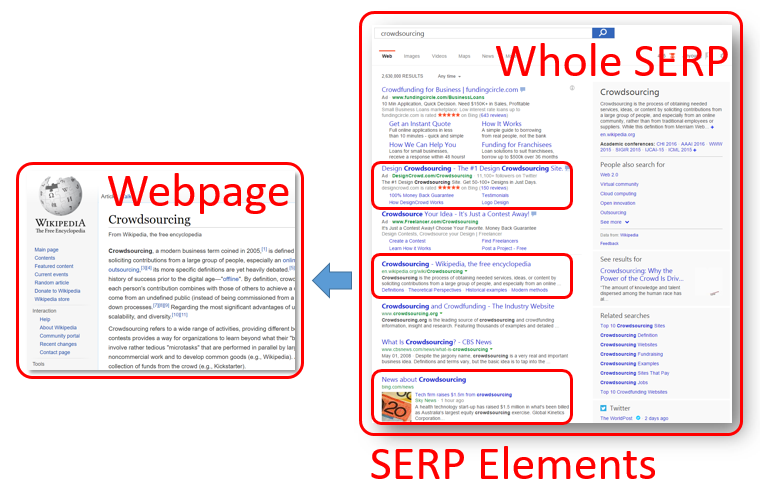
\includegraphics[scale=0.5]{images/judging_units}
		\caption{Various judging units for web search results.} 
		\label{fig:judging_units}
	\end{center}
\end{figure}

Basically, judging unit should be determined by the goal of evaluation: if you care about the quality of ranked list, collecting judgment for each web search result seems like a natural choice. If the presentation of SERP is primary concern, SERP should be the right unit for judgment. 

On the other hand, if the judging target is reasonably complex with multiple sub-components, it is also possible to collect judgments at smaller unit (i.e., SERP elements) and then calculate scores for large unit (i.e., whole SERP) by combining unit scores in a sensible way. This is how most of IR evaluation metrics (i.e., MAP or NDCG) works.

Now, if we want to collect judgment for SERP, should we collect element-wise judgments and then combine, or collect single SERP-level judgment? This question can be generalized into the decision of judging unit when the judging target is complex. In fact, there is no hard and fast rule in determining right judging unit, but here we describe a few trade-offs. 

Smaller judging unit means simpler judging task which can be faster and more reliable individual judging task. However, the number of judgments to evaluate larger judging unit (i.e., SERP) can be quite high if the judging unit is small, making overall judging cost higher than collecting a single judgment for larger judging unit.

Smaller judging unit also means better reusability of individual labels, because you can combine labels for each SERP element to evaluate arbitrary SERP configuration. This means that the cost of collecting judgments can be amortized over multiple experiments. In fact, query-URL relevance judgment has been so widely used in TREC and other settings because it allows the creation of test collection which can be used to evaluate any ranked list.

On the other hand, smaller judging unit makes an assumption that each label can be collected independent of other element. This is hardly true in a typical search scenario where the concept and criteria of relevance can evolve over time. On this regards, larger judging unit has the benefit of providing rich context for judges. Also, larger judging unit can capture the interaction between elements -- i.e., redundancy among documents in a ranked list.

In literature, as briefly mentioned above, document-level judgment is most prevalent. However, there has been a few papers which deal with SERP-level evaluation. \cite{Bailey2010} introduces a judgment scheme which can capture the interaction among SERP elements as well as element-level quality. 

SERP-level judgments were introduced in \cite{Thomas2006}, where they used pairwise judging in order to minimize the complexity of defining judging criteria. (more about this in the following section) Several other works including  \cite{Kim:2013} refined this idea to include dimensional relevance judgments as well as overall SERP-level comparison.
% \cite{Al-Maskari2007} and

\subsubsection{Absolute vs. Relative Judgment}
Another consideration in determining a judging target is the type of judgment, which can be either absolute or relative. In absolute judgment judgment is collected for a single judging target, whereas relative judgment asks for pairwise preference between two judging targets. Figure \ref{fig:judgment_types} shows two types of judgments in evaluating web search results.

\begin{figure}
	\begin{center}
		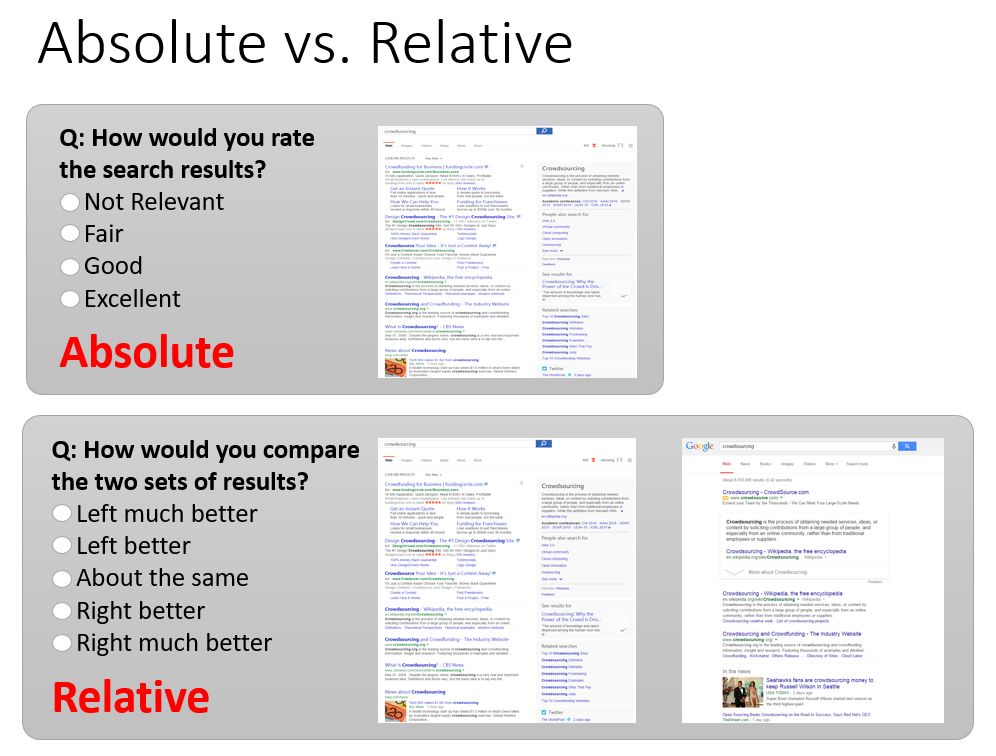
\includegraphics[scale=0.5]{images/judgment_types}
		\caption{Absolute vs. Relative judgments} 
		\label{fig:judgment_types}
	\end{center}
\end{figure}

Now, how should one choose between absolute vs. relative judgment? In general, making an absolute scale judgment requires having objective criteria among different levels, whereas relative judgment can avoid the issue. \cite{CarteretteBCD08} also suggested that relative judgment is more accurate for document-level judging.

Relative judgment has been used in various evaluation settings. \cite{Chandar2013} employed document-level pairwise judging using another document as a context, with a goal of novelty and diversity evaluation. \cite{Arguello:2011} also proposed an evaluation scheme for aggregated search based on pairwise preference judgment at element-level. \cite{Zhou:2012} used SERP-level pairwise preference judgment as a part of the evaluation framework for aggregated search.

On the other hand, absolute judgments are reusable in that you can compare among any items for which you have item-level labels, whereas you need to collect labels for every pair of items. Therefore, if you want to reuse judgments in a production environment where multiple generations of ranking techniques should be compared against each other, absolute judgment might save the cost in the long run. This is also the reason that TREC has employed absolute judgment since its inception.


\subsection{Judging Criteria}
The central assumption of offline evaluation is that human judges can represent real users, and we often want judges to tell us if the judging target would be useful to the potential user. However, it is not a trivial task for judge given contextual and multi-faceted nature of relevance. (\cite{Borlund:2003})

\newpar
Effort based judgments \cite{Yilmaz:2014} \cite{VermaYC16}

\newpar
Relevance vs. Usefulness-based evaluation \cite{Zhou:2012} \cite{Kim2016}

\newpar
Novelty and diversity \cite{Chandar2013}

\newpar
Multi-dimensional judgment collection \cite{Golbus:2014:CDR} \cite{Kim:2013}


\subsection{Additional Issues}

\newpar
Judging scale \cite{Turpin2015} \cite{Jarvelin:2002}

\newpar
Decision Criteria

- Judgment goal (target / decision)

- Judging effort/time

- Outcome reliability/intepretability

- Reusability

\section{Collecting Judgments}

Choosing Judges: 

- Crowd vs. Expert \cite{Kazai:2013} \cite{Alonso20121053}

- Query owner vs. non-owners \cite{Chouldechova:2013}

\newpar
Reducing noise in judging: 

- Anchoring bias in judging \cite{Shokouhi:2015}

- Multiple judgments and majority voting, etc. \cite{Venanzi:2014}

\cite{aroyo2013measuring} \cite{aroyo2013crowd}

\newpar
Efficient judgment collection using Crowdsourcing

- Design decisions that need to be tackled  \cite{Blanco:2011} \cite{Kazai2012} \cite{Alonso2012} \cite{Alonso:2015} \cite{Scholer:2013} 

- Incentivising judges and how to make it more attractive (payment / I/F)
\cite{Megorskaya2015} \cite{Davtyan2015}  \cite{Rokicki:2014}  \cite{Eickhoff:2012}

\section{Open Issues}

Collecting labels for contextual / personalized search results

- using judgments with search context?

\newpar
Collecting labels for whole SERP / non-document results

\newpar
Collecting labels for non-traditional endpoints (i.e., conversational agent)

- Judgment for Desktop vs. Mobile environment \cite{Verma:2016:CRMD}

\newpar
Session/Task-based evaluation \cite{Moraveji:2011} \cite{Xu:2009}


\chapter{Evaluation Metrics}
\label{c-metrics}

The second step in offline evaluation is selecting or designing a meaningful evaluation metric. This is essentially the question of how to combine labels to meaningful numbers. For traditional IR evaluation where the labels are collected at query-URL level, combining labels to a metric requires quite a few assumptions, or even a user model. In this chapter, we go over the various considerations of IR metric design, as well as the user models behind these metrics. We briefly survey some established metrics but spend more time on recent developments: explicit models of user behavior, deriving metrics from these, and open issues including session-level measurement, dealing with variation, and considering rich SERPs. (20-25 pages)

\section{Basic IR evaluation metrics}

- Metrics based on absolute judgments (e.g. \cite{cooper73selecting})

- Metrics based on preference-based judgments, including e.g.\ aggregated in-situ side-by-side \cite{Thomas2006}

- Ranking-based metrics (Tau/TauAP)

- Criticisms: especially reproducability/replicability

\section{Metrics based on simple aggregation of labels/qrels}

- Set-based: P, R

- Rank-based: P@$k$, AP, RR

- Criticisms: what tasks and behaviors are modeled here?

\section{Models of behavior}

Evaluation metrics that are based on explicit models of user behavior

- The cascade model and variants

- Weights, the C/L/W framework \citep{Moffat2013}

- ERR, EBU, GAP, Time-biased gain, etc.

- Weighted precision metrics such as RBP, INST; notion of residual \citep{Moffat08,Moffat15}

- $\alpha$-NDCG, IA metrics, etc.

- Cost-based/economic models and the prospects of metrics from these

- Session-level metrics \cite{kanoulas2011evaluating} \cite{Järvelin2008}

\section{Model fitting}

Fit of metrics to models; estimating the distribution of parameters/metric values based on user data

\cite{CarteretteKY11}, \cite{Moffat2013}

\section{Open issues}

Open issues in behavior models and the corresponding metrics

- Whole-page quality

- Caption effects

- Variation between users: behaviors, learning styles, cognitive styles, topic expertise, search system expertise, expectations of the system, query variation, \dots

- Duplication in SERPs

- Learning (?)

- Non-traditional tasks and novel UIs

- Choosing between metrics; sensitivity; finding evidence any of them correlates with user behavior or other important dependent variables

- Measuring things outside the SERP: query formulation, source/engine selection

\chapter{Experiments}
\label{c-experiment}

Experiments is defined as the collection of labels and metrics defined on top of them. We first look over many considerations in order to design an experiment given a budget and time constraint. We then focus on a set of analyses we can perform once the data is collected, followed by the ways of reporting experimental results. (\ensuremath{\approx} 15 pages)

\section{Designing an Experiment}

- How to select queries?

- How many queries? \cite{Sakai:2014}

- How many documents? \cite{CarterettePFK09}

- How to distribute judgment efforts across queries and documents? \cite{CarterettePKAA09, YilmazR09}


\section{Analysis of Experimental Results}

Survey of research results \cite{Sakai:2016}

Drawing conclusions from metrics 

- Hypothesis Testing \cite{Dincer:2014}

- Comparison of different types of significance tests \cite{SmuckerAC09}

\newpar
Various analysis methods

- Power analysis \cite{Sakai:2014}

- Failure analysis

- Sensitivity and Reliability analysis \cite{Urbano:2013} 

- Informativeness (MaxEnt) \cite{AslamYP05}

- ETC \cite{Bron:2013} \cite{Boytsov:2013}  \cite{Robertson:2012}

\newpar
Reporting results

- Effect sizes and distributions, vs point estimates and $p$ values

\section{Open Issues}

- Reusability for SERP/task-level evaluation

- Beyond significance testing -- bayesian alternatives?

- Reusability / Generalizability of experimental results


\chapter{IR Evaluation in Practice}
\label{c-practice}

In this chapter, we review evaluation practices happening in both academia and industry. We first cover evaluation practices from academia, including recent TREC tracks, data generation efforts. We also look at evaluation efforts in related area such as recommendation systems and conversational agents. We then turn to evaluation practices from industry including major players in search and recommendation based on published papers and articles.

\section{Evaluation Practices from Academia}

Emerging TREC tracks

- Task track

- Microblog track

- Live QA track

- Contextual suggestions track

\newpar
Dataset generation efforts

- Living labs for IR \footnote{http://living-labs.net/}

- Data set shared by industry \footnote{http://jeffhuang.com/search\_query\_logs.html}

\newpar
Evaluation in related domains

- Aggregate search \cite{Zhou:2013}

- Recommendation systems \cite{gunawardana2015evaluating}

- Conversational agents

\section{Evaluation Practices from Industry}

How are the practitioners doing? (\ensuremath{\approx}15 pages)

- Google \footnote{How Search Works (Google) https://www.google.com/insidesearch/howsearchworks/thestory/} \footnote{Updating Our Search Quality Rating Guidelines
	 https://webmasters.googleblog.com/2015/11/updating-our-search-quality-rating.html}

- Bing \footnote{The Role of Content Quality in Bing Ranking (Bing)
	 http://bit.ly/1T1BaYN}

- Netflix \cite{Gomez-Uribe2015}  \footnote{The Netflix Tech Blog: Learning a Personalized Homepage
	http://techblog.netflix.com/2015/04/learning-personalized-homepage.html}

- Facebook \footnote{Who Controls Your Facebook Feed (Slate) http://slate.me/1T1BbvU}

- Pinterest \footnote{Machine Learning at Pinterest http://www.slideshare.net/HiveData/the-hive-think-tank-machine-learning-at-pinterest-by-jure-leskovec-61383413}

- LinkedIn \footnote{http://www.slideshare.net/dtunkelang/search-quality-at-linkedin}

- Startups \footnote{The Humans Hiding Behind the Chatbots http://www.bloomberg.com/news/articles/2016-04-18/the-humans-hiding-behind-the-chatbots}

\footnote{10 Data Acquisition Strategies for Startups http://bit.ly/28IHlC7}

\newpar
Common features: combine online and offline evaluation

- Offline evaluation for early iteration

- Online evaluation for final ship decisions

\chapter{Conclusions}

In this chapter we conclude this survey by providing the summary of contents so far. 
We also provide a brief outlook toward the future of offline evaluation for IR.

\section{Summary}

Recap: general Components of Offline Evaluation

-	Experiment

-	Search Task (Query / context)

-	Evaluation Metric

-	Judging Method (Interface / rating scale) 


\section{Future of Offline Evaluation for IR}

Emerging trends in the tech ecosystem

- Mobile-first: different interfaces and information needs

- Natural-language interaction: Bots and Conversational agents

- End-to-end support for task completion: e.g., restaurant reservation 

\newpar
Future of Offline Evaluation

- Evaluation of search agents (as well as engines)

- Evaluation of various information 'cards'

- Evaluation of end-to-end task completion

\newpar
Future of Offline Evaluation Research

- Need for Academy-Industry collaboration

\backmatter  % references

\bibliographystyle{plainnat}
\bibliography{ch1_intro,ch1_user_study,ch2_judgment,ch2_crowdsourcing,ch3_metrics,ch4_experiment,ch5_industry}
	
\end{document}
